\chapter{Physical Setup}\label{ch:physsetup}
\section{Pumps}
\todo[color=03physicalSetup]{talk more about the pumps used, because the only reason we use them is: "they are present in the setup", e.g. we don't care why other pumps are not as good. [debatable]}
Simply put, a pump is device used to move liquid through a piping system and to raise the pressure of the liquid. We will focus on explaining 
and describing only centrifugal pumps, since this is the type of pump present in our setup. 
\subsection{Principle}
Centrifugal pumps are the most commonly used type of pump, due to its simple construction, relative low 
cost, reliability and quiet operation.

When the pump is in operation, an increase in the fluid pressure from the pump's inlet to its outlet is created.
This pressure difference drives the fluid further through the system.

The pump creates a pressure difference by transferring mechanical energy from the motor to the fluid through the impeller. 
The fluid flows from the inlet to the impeller center and out along its blades. The centrifugal force increases
the fluid velocity and consequently the kinetic energy is transformed to pressure. 

The blades of the rotating impeller transfer energy to the fluid by increasing velocity and pressure.
The fluid is sucked into the impeller at the impeller eye and flows through the impeller channels formed by the blades between the shroud and hub.

The design of the impeller depends on the requirements for application, pressure and flow. The impeller is the primary component 
determining the pump performance. Pumps variants are often created only by modifying the impeller.

\newpage
Figure \ref{fig:pump_sections} represents the cross section and the transverse section of a centrifugal pump.
\begin{figure}[h]
    \centering
    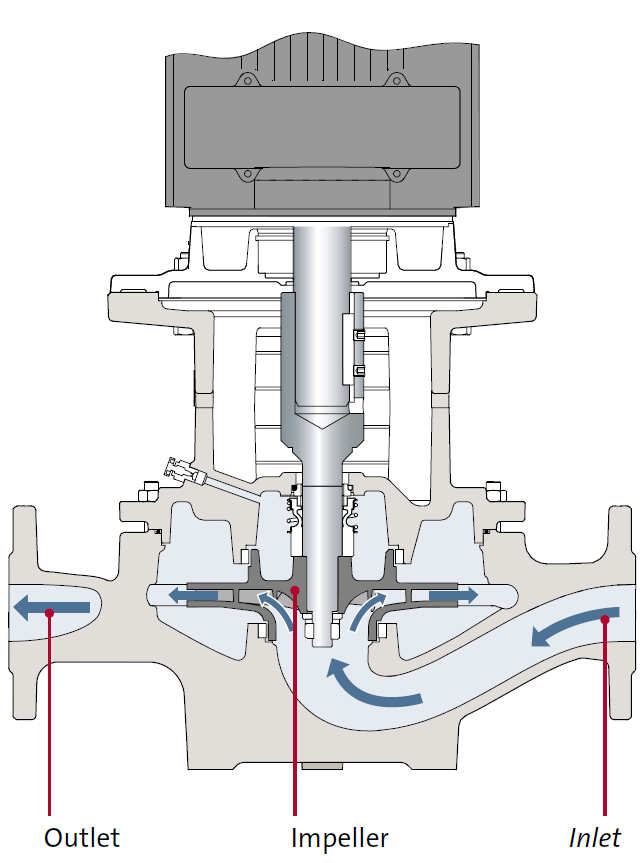
\includegraphics[width=0.4\linewidth]{figures/pump_cross_section.PNG}
    \qquad
    \hfill
    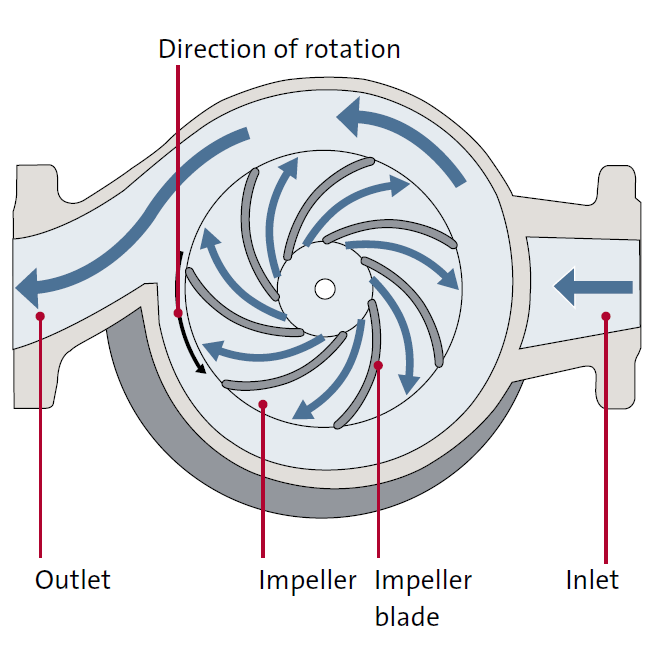
\includegraphics[width=0.4\linewidth]{figures/pump_above_view.PNG}
    \caption{Centrifugal Pump}
    \label{fig:pump_sections}
\end{figure}

\subsection{Affinity Laws}
Affinity laws are mathematical relationships that provide a way to estimate the changes in performance of a pump, as a result
of a change in one of the basic pump variables.
In it's simplest form, the term law, means a principle that has been proven true for all cases.
\todo[color=03physicalSetup]{"proven true for all cases"? that can't be correct for an estimate}

\begin{align}
	\left(\frac{N_1}{N_2}\right)^1 = \frac{Q_1}{Q_2} &&
	\left(\frac{N_1}{N_2}\right)^2 = \frac{H_1}{H_2} &&
	\left(\frac{N_1}{N_2}\right)^3 = \frac{P_1}{P_2}	
\end{align} 
Equations for constant impeller diameter $D$ \cite{Volk2014}


\begin{align}
	\left(\frac{D_1}{D_2}\right)^1 = \frac{Q_1}{Q_2} &&
	\left(\frac{D_1}{D_2}\right)^2 = \frac{H_1}{H_2} &&
	\left(\frac{D_1}{D_2}\right)^3 = \frac{P_1}{P_2}	
\end{align} 
Equations for constant rotational speed $N$ \cite{Volk2014}
\newpage

\subsection{Performance Curves}
\subsubsection{Pump Head Curve}
A QH-curve or pump curve defines the head as a function of the flow. The flow is the rate of the fluid going through the 
pump. It is generally stated in cubic meter per hour $[m^{3}/h]$. Figure \ref{fig:pump_head_curve} represents a typical pump head curve.


\begin{figure}[h]
	\centering
	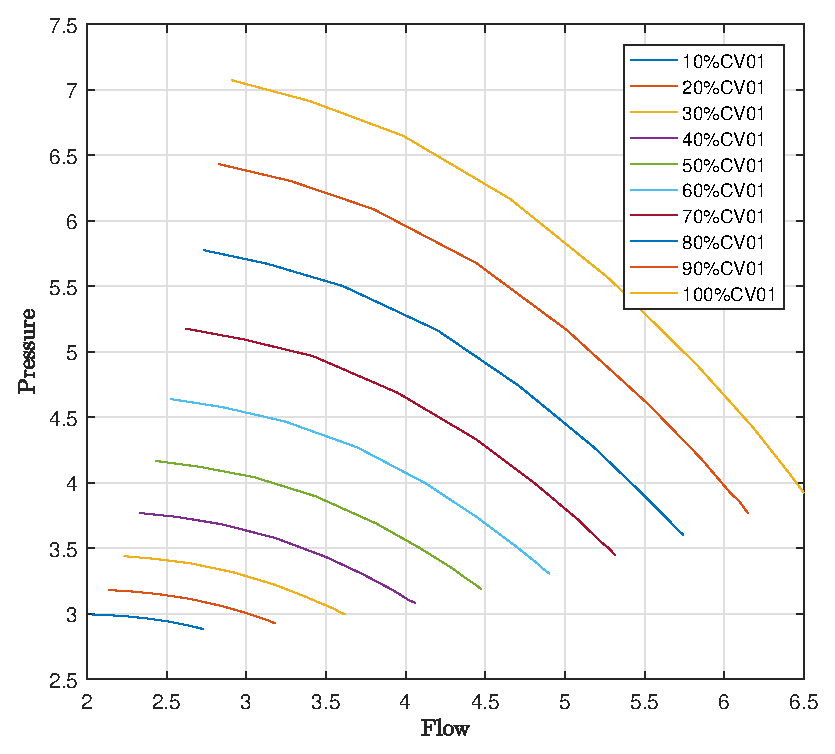
\includegraphics[width=0.4\textwidth]{figures/05mathematicalModeling/pumpCurves.eps}
	\caption{Pump Head Curve}
	\label{fig:pump_head_curve}
\end{figure}
\todo[color=04mathematicalModelling]{either show a curve or say points}


\subsubsection{System Head Curve}
A system head curve is a graphical representation of the pump head that is required to move fluid through a piping system at various flow rates.
The system curve helps quantify the resistance in a system due to friction and elevation change over the range of flows.

Simply put, the system curve shows how much resistance the pump has to overcome in order to be able to move a certain amount of fluid though the system.
As stated before, the resistance can come from friction with the pipes, or elevation changes.
\todo[color=04mathematicalModelling]{repetitive, choose one that you think explains it the best}
\todo[color=04mathematicalModelling]{insert system curve photo}


\section{Pipes}
Pipes are a way of transporting liquids or gasses, inside a controllable environment.
They are used to interconnect the pumps and the tank and other peripherals.
One common analogy compares them to wires in electrical circuits.

Based on their diameters, material and shape,
they introduce resistance to the flow of the pumped medium.
Staying with the analogy to electrical circuits,
this can be compared to the cross sectional area and the specific resistance of a wire material.

\section{Valves}
A valve is a device used to regulate the flow of a gas or liquid through a piping system.
The valve built into our system is not used for regulatory purposes,
but only to simulate disturbances in the system.
Valves can be actuated by different means, such as air pressure, electric motors or rotary handles.

\section{Sensors}
To be able to monitor the system closely, different sensors are used.
\todo[color=03physicalSetup]{write about the sensors used in the system}

\subsection{Flow Meter}
\subsection{$\Delta$Pressure Sensor}
\subsection{Power Sensor}
\todo[color=03physicalSetup]{complete this list of subsections}
\todo[color=03physicalSetup]{maybe take out of ToC? (subsection*)}

\todo[color=03physicalSetup]{Do we want a section about xPC and Simulink Realtime?}
